%%%%%%%%%%%%%%%%%%%%%%%%%%%%%%%%%%%%%%%%%%%%%%%%%%%%%%%%%%%
% --------------------------------------------------------
%  _____           
% |_   _|_ _ _   _ 
%   | |/ _` | | | |
%   | | (_| | |_| |
%   |_|\__,_|\__,_|
%
% LaTeX2e Template
% Version 2.6.0 (21/04/2026)
%
% Author: 
% Guillermo Jimenez (memo.notess1@gmail.com)
% 
% License:
% Creative Commons CC BY 4.0
% --------------------------------------------------------
%%%%%%%%%%%%%%%%%%%%%%%%%%%%%%%%%%%%%%%%%%%%%%%%%%%%%%%%%%%
% --------------------------------------------------------
% Github Repository:
% https://github.com/MemoJimenez/Tau-class
% --------------------------------------------------------
%%%%%%%%%%%%%%%%%%%%%%%%%%%%%%%%%%%%%%%%%%%%%%%%%%%%%%%%%%%

\documentclass[9pt,a4paper,twocolumn,twoside]{tau-class/tau}
\usepackage[english]{babel}
\setlength{\eqskip}{13pt}

% Spanish babel recomendation
% \usepackage[spanish,es-nodecimaldot,es-noindentfirst]{babel} 

%----------------------------------------------------------
% Title & Authors/Affiliations
%----------------------------------------------------------

\doctype{CS240 Proposal}
\title{Penalized Value-Connection Model for Shanghai Metro Line Planning}

%----------------------------------------------------------

\author[a,1]{Yuzhou Lu}
\author[a,2]{Zaizhou Yang}
\author[a,3]{Jingrong Guan}

%----------------------------------------------------------

\affil[a]{ShanghaiTech University}

%----------------------------------------------------------
% Document-, Footer- information
%----------------------------------------------------------

\dates{This manuscript was compiled on \today}

\docinfo{CS240 project proposal on graph optimization for urban rail transit planning.} 

%----------------------------------------------------------

\footinfo{CS240 Proposal}
\theday{\today}
\organization{ShanghaiTech University}
\leadauthor{Y. Lu et al.}

%----------------------------------------------------------
% Abstract and Keywords
%----------------------------------------------------------

\begin{abstract}    
    This project studies a graph-optimization formulation for Shanghai metro line planning. Given candidate stations and their values, the planning task is to design one or more routes that connect valuable urban centers while penalizing construction length, sharp turns, and excessive open endpoints. The reward between two connected stations is modeled as the product of their values divided by their shortest-path distance in the selected metro network, which favors spatially efficient connections among high-value areas. The goal is to generate candidate rail corridors that are interpretable, computationally tractable, and compatible with practical planning constraints.
\end{abstract}

%----------------------------------------------------------

\keywords{transit network design problem, penalized network design, metro planning, candidate stations, Shanghai}

%----------------------------------------------------------

\begin{document}
		
    \maketitle 
    \thispagestyle{firststyle}
    
%----------------------------------------------------------

\section{Topic Selection}

    \taustart{N}etwork design is one of the most strategic and difficult stages in urban rail transit planning. The spatial structure of a metro network determines which areas can be reached directly, where transfers are required, and how efficiently demand can be served, while also constraining later decisions such as frequency setting and timetable design. This challenge is commonly studied as the Transit Network Design Problem (TNDP), a constrained and computationally difficult problem because cost, accessibility, coverage, and service quality often conflict with one another \cite{owais2026tndp}.

    In this project, we study a simplified but meaningful version of metro line planning in a selected Shanghai study area. The core problem is: given a set of candidate stations and a scalar value for each station, design routes that connect selected stations and maximize our penalized value-connection objective. The candidate stations are generated from several urban-data layers, with the detailed selection and merging process described in Section~\ref{sec:data-collection}. We therefore focus the optimization stage on route design over a prepared candidate set, rather than on detailed ridership forecasting or professional engineering design.



\section{Problem Formulation}

    We formulate the planning task as a penalized value-connection problem on a spatial graph. The input of the optimization stage is a set of candidate stations
    \[
        V = \{1,2,\ldots,n\}.
    \]
    Each candidate station $i \in V$ has a coordinate $p_i=(\lambda_i,\phi_i)$ and a nonnegative value $v_i$. The station set and values are produced by the data collection process in Section~\ref{sec:data-collection}. The formulation below treats them as the input to the route-design problem.

    We construct a complete candidate graph $G=(V,E)$, where each candidate edge $e=(i,j) \in E$ has construction length $\ell_{ij}$, measured by the geographic distance between its two endpoint stations. The planning decision is not only to select a set of edges, but to select a set of metro lines
    \begin{equation}
        \mathcal{L}=\{L_1,L_2,\ldots,L_K\}.
    \end{equation}
    Each line $L_k$ is an ordered sequence of candidate stations. It may be an open line, such as $(s_1,s_2,\ldots,s_m)$, or a closed loop line, such as $(s_1,s_2,\ldots,s_m,s_1)$. Therefore, cycles are allowed in the planned network. The selected metro subgraph $S=(V_S,E_S)$ is the union of all stations and edges used by the lines in $\mathcal{L}$. Let $x_{ij} \in \{0,1\}$ indicate whether edge $(i,j)$ is selected by at least one line, $y_i \in \{0,1\}$ indicate whether station $i$ is included, and $z_{ij} \in \{0,1\}$ indicate whether stations $i$ and $j$ are both included in the same connected selected network.

    For any two selected stations $i,j \in V_S$, let $D^S_{ij}$ denote the shortest-path distance between $i$ and $j$ within the selected metro subgraph $S$, where the length of a path is the sum of the construction lengths $\ell_e$ of all selected edges $e$ on that path. Thus $D^S_{ij}$ is not the direct geographic distance between $i$ and $j$ unless the selected network contains a direct edge between them. The key modeling assumption is that connecting two high-value stations is more beneficial when they are close in the planned metro network. Therefore, if stations $i$ and $j$ are included in the same connected planned line or network, their pairwise reward is defined as
    \begin{equation}
        r_{ij}(S) = \frac{v_i v_j}{D^S_{ij}}, \qquad i,j \in V_S,\ i<j .
    \end{equation}
    The product $v_i v_j$ captures the idea that two strong urban centers are more valuable to connect, while the division by $D^S_{ij}$ favors planned networks in which valuable station pairs can reach each other through short metro paths.

    We no longer impose a hard total construction-length budget. Instead, construction length enters the objective as a soft cost. Let
    \begin{equation}
        C(S)=\sum_{(i,j)\in E} \ell_{ij}x_{ij}
    \end{equation}
    be the total construction length of the selected metro subgraph.

    To discourage unrealistic rail alignments, we introduce a line-level turn-angle penalty. This penalty is computed along each ordered line rather than from the unordered adjacency structure of the selected subgraph. For every consecutive triple of stations $(a,b,c)$ on the same line, let $\theta_{abc}$ denote the deflection angle at station $b$, where $\theta_{abc}=0^\circ$ corresponds to a straight continuation and larger values correspond to sharper turns. For a closed loop line, triples are evaluated cyclically across the connection from the last station back to the first station. For an open line, only interior stations contribute to the turn penalty; terminal stations do not.
    \begin{equation}
        T(\mathcal{L}) =
        \sum_{L_k \in \mathcal{L}}
        \sum_{(a,b,c)\in T(L_k)}
        \left(
        \frac{\max(0,\theta_{abc}-\theta_0)}{90}
        \right)^2 .
    \end{equation}

    We also penalize open terminal endpoints in the selected subgraph. Let
    \begin{equation}
        d_i(S)=\sum_{j:(i,j)\in E} x_{ij}
    \end{equation}
    be the degree of station $i$ in the selected metro subgraph. The endpoint count is
    \begin{equation}
        P(S)=\sum_{i\in V} y_i\,\mathbf{1}\{d_i(S)=1\}.
    \end{equation}
    This term is not a hard upper bound on the number of lines. Instead, it is a soft topological penalty: a simple open line contributes two endpoints, while many disconnected or branching terminal spurs contribute more endpoints. Penalizing $P(S)$ therefore discourages an unrealistically large number of open line termini and gives the objective a way to prefer more compact line structures when the added station reward is not large enough.

    The final objective is
    \begin{equation}
        \max \quad
        \sum_{\{i,j\}\subseteq V}
        \frac{v_i v_j}{D^S_{ij}} z_{ij}
        - \lambda_1 C(S)
        - \lambda_2 T(\mathcal{L})
        - \lambda_3 P(S)
    \end{equation}
    subject to line-consistency and connection constraints, including
    \begin{equation}
        z_{ij} \leq y_i,\qquad
        z_{ij} \leq y_j,\qquad
        \forall i,j \in V,\ i<j,
    \end{equation}
    together with consistency constraints requiring that every selected edge belongs to at least one line in $\mathcal{L}$ and that every selected station with $y_i=1$ appears on at least one selected line. The union subgraph $S$ may contain cycles, either because an individual line is a closed loop or because multiple lines jointly create a cycle. If the model is restricted to a single open line, then the result is a path; if closed or multiple lines are allowed, the result can be a cyclic rail network.

    In words, the model asks: given candidate stations with coordinates and values, which set of open or closed metro lines should be built so that the connected high-value station pairs produce the largest total reward after accounting for construction length, excessive local turns, and unnecessary open termini? This formulation keeps the project close to classical network design, orienteering, and prize-collecting problems.

    \section{Related Work}

    Laporte et al. study the location of a single rapid-transit alignment as a maximal trip-coverage problem \cite{laporte2005tripcoverage}. Their model selects an ordered set of stations under a maximum line length and non-self-intersection constraints. Algorithmically, they solve the NP-hard problem with constructive heuristics, especially greedy extension, greedy insertion, and post-optimization local improvement. This work is the closest single-line reference for our project: our model also searches over candidate stations, but replaces the hard length budget with a construction-cost penalty and uses station values to define connection reward.

    Chai et al. formulate urban rail network design under road-network, travel-demand, and land-use constraints \cite{chai2019urbanrail}. Their method builds a restricted basic network, defines station-importance and spatial-matching indices, and then applies a simulated annealing algorithm with neighborhood moves on lines and sections. Compared with this full network-design formulation, our project keeps the same spirit of spatially constrained rail planning but simplifies the inputs to candidate-station values, route geometry, and construction length, making the algorithm easier to implement and evaluate within the course scope.

    Ahmed et al. propose an integrated GIS and genetic-algorithm framework for rail transit system planning \cite{ahmed2020gisga}. The paper first screens feasible station and corridor locations from spatial, demographic, economic, environmental, and topological layers, and then uses a genetic algorithm to optimize station selection and line layout jointly, with shortest-path computation used inside the fitness evaluation. This motivates our own separation between spatial preprocessing and graph optimization: we construct a candidate-station set from public urban data, then solve a smaller penalized value-connection problem instead of a full life-cycle planning model.

\section{Data Collection and Station Selection}
    \label{sec:data-collection}

    The data pipeline converts public spatial data from central Shanghai into a discrete candidate-station set. The raw geographic data is downloaded from OpenStreetMap through the Overpass API. From these OSM features, we extract four layers of urban centers: residential population centers, estimated job centers, transport centers, and large commercial centers. These layers are not treated as final stations directly. Instead, they provide weighted evidence about where a station may be valuable.

    Residential population centers are derived from building footprints and housing-related tags. Population is distributed to residential building centroids and then clustered by weighted $k$-means. Job centers are estimated from functional urban features such as offices, retail and service areas, education, healthcare, industry, and hotels; these features are assigned approximate employment values and clustered in the same way. Transport centers are extracted from major railway and public-transport features, while commercial centers are selected from large shopping and activity attractions. Together, these layers describe where people live, where they work, where they transfer, and where they gather.

    \begin{figure*}[t]
        \centering
        \begin{minipage}{0.49\textwidth}
            \centering
            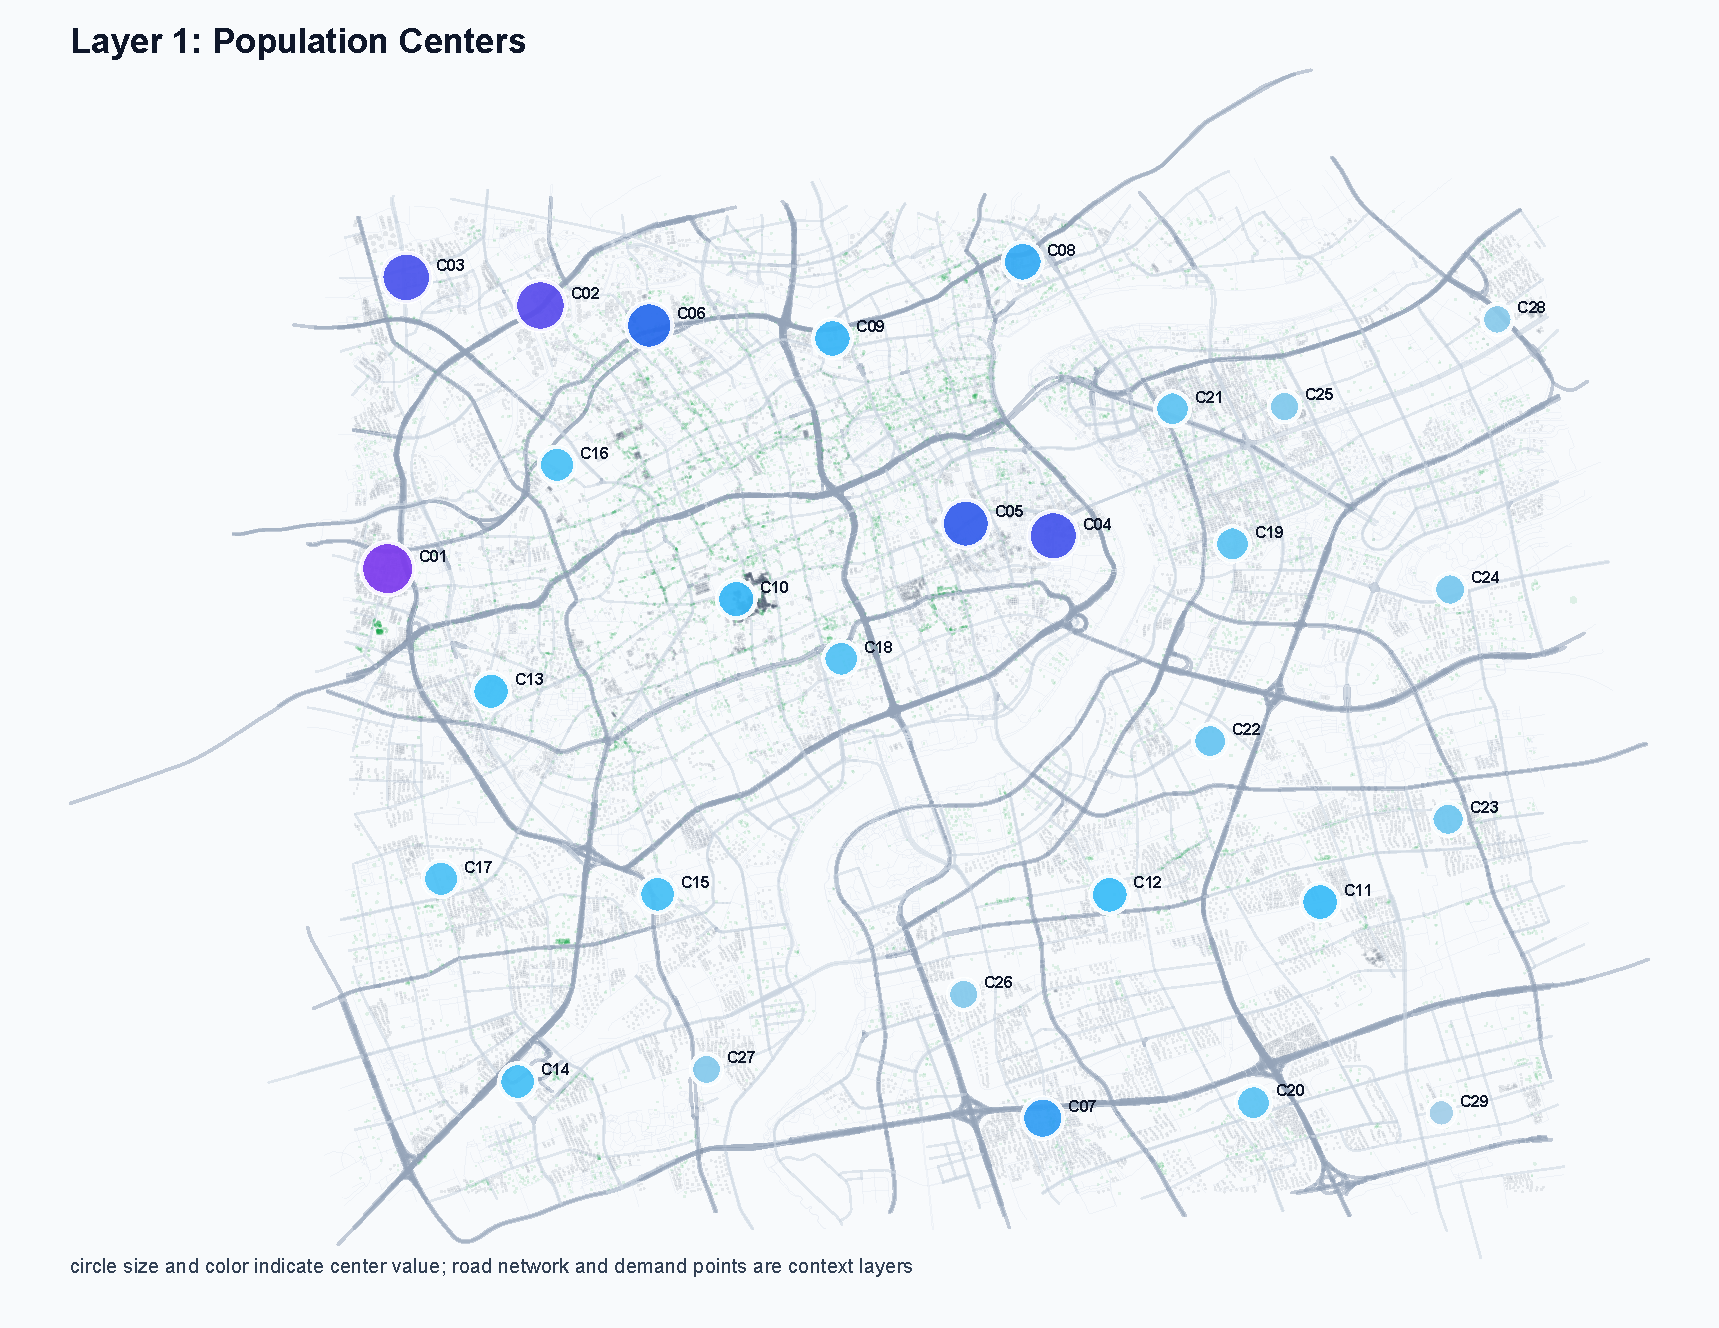
\includegraphics[width=\linewidth]{figures/01a_population_centers.pdf}
            \caption*{(a) Residential population centers}
        \end{minipage}
        \hfill
        \begin{minipage}{0.49\textwidth}
            \centering
            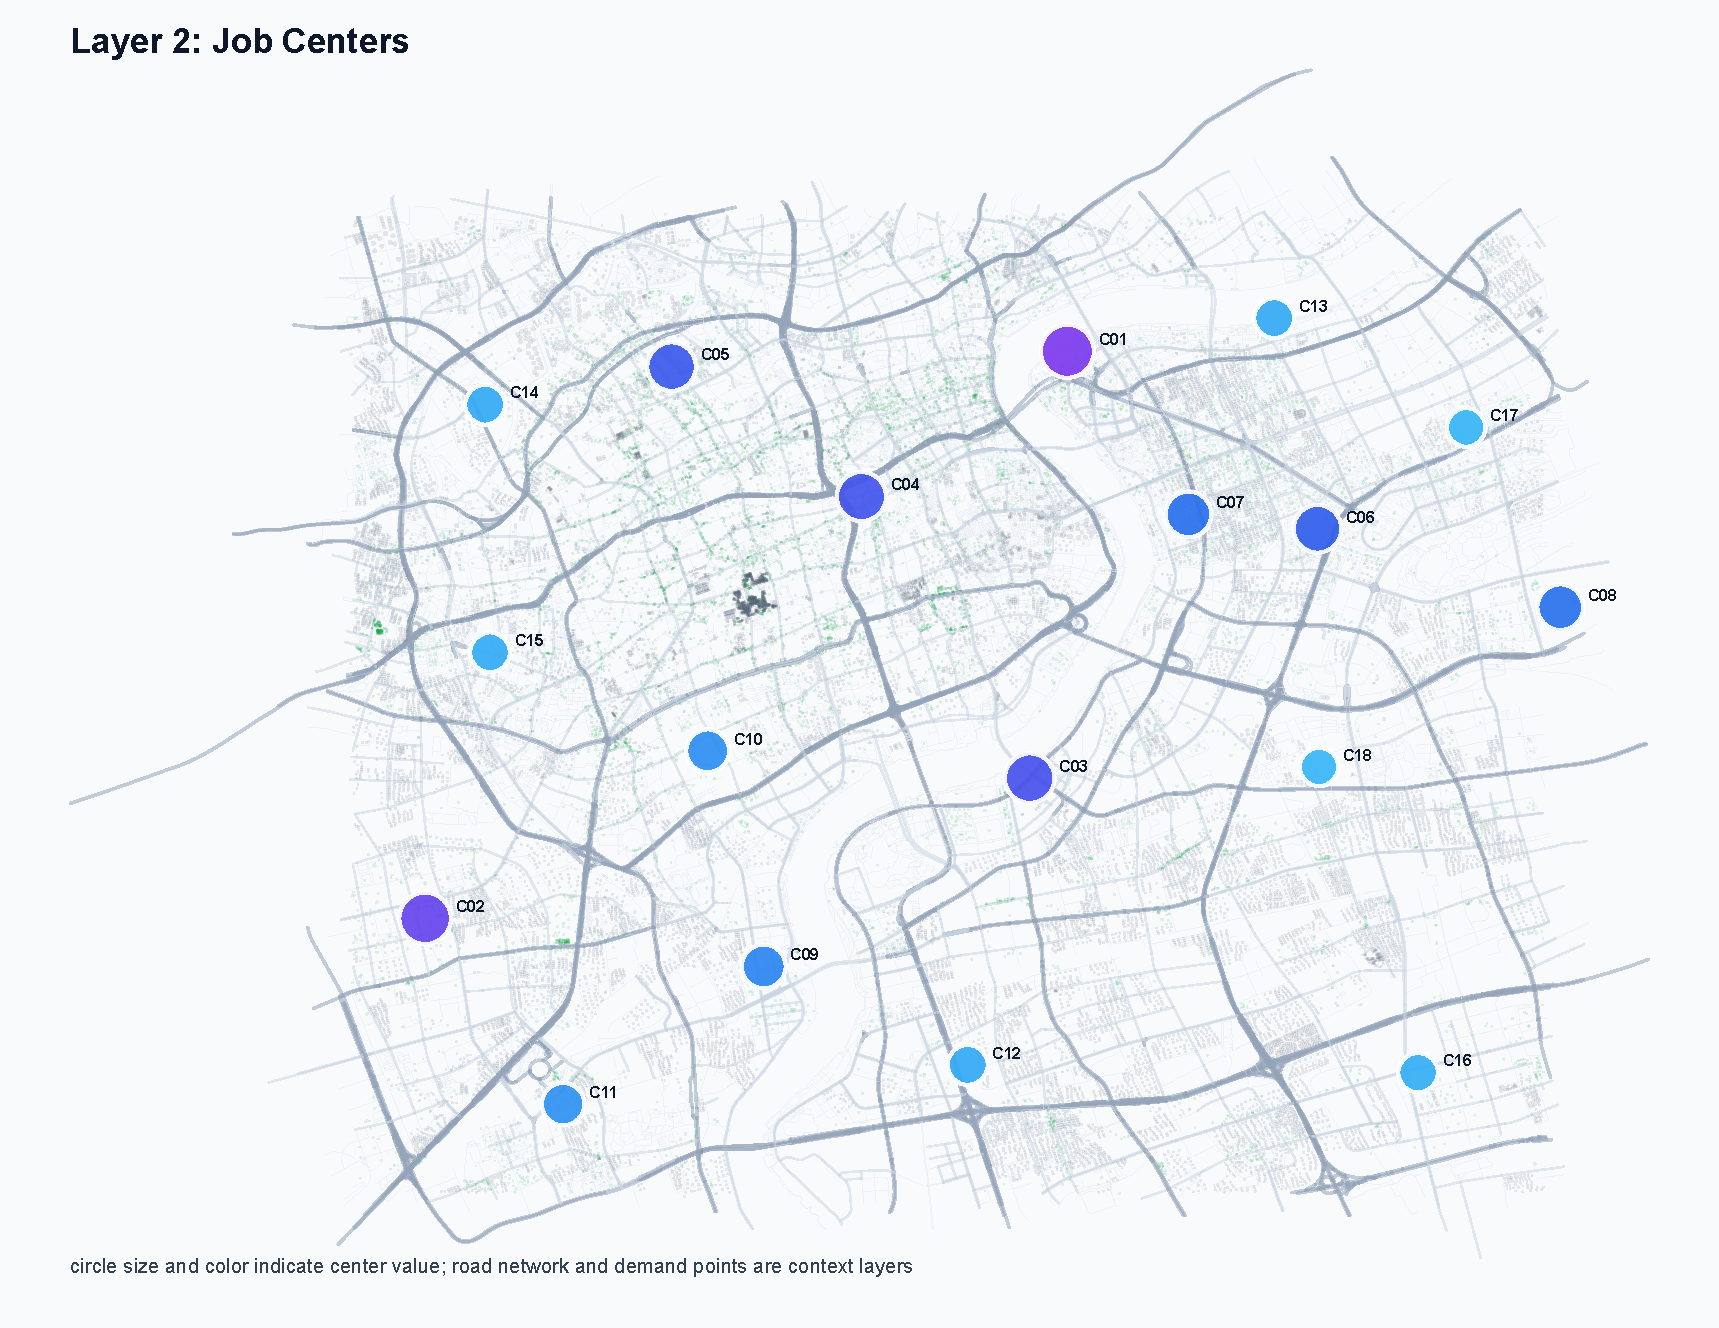
\includegraphics[width=\linewidth]{figures/01b_job_centers.pdf}
            \caption*{(b) Estimated job centers}
        \end{minipage}

        \vspace{0.6em}
        \begin{minipage}{0.49\textwidth}
            \centering
            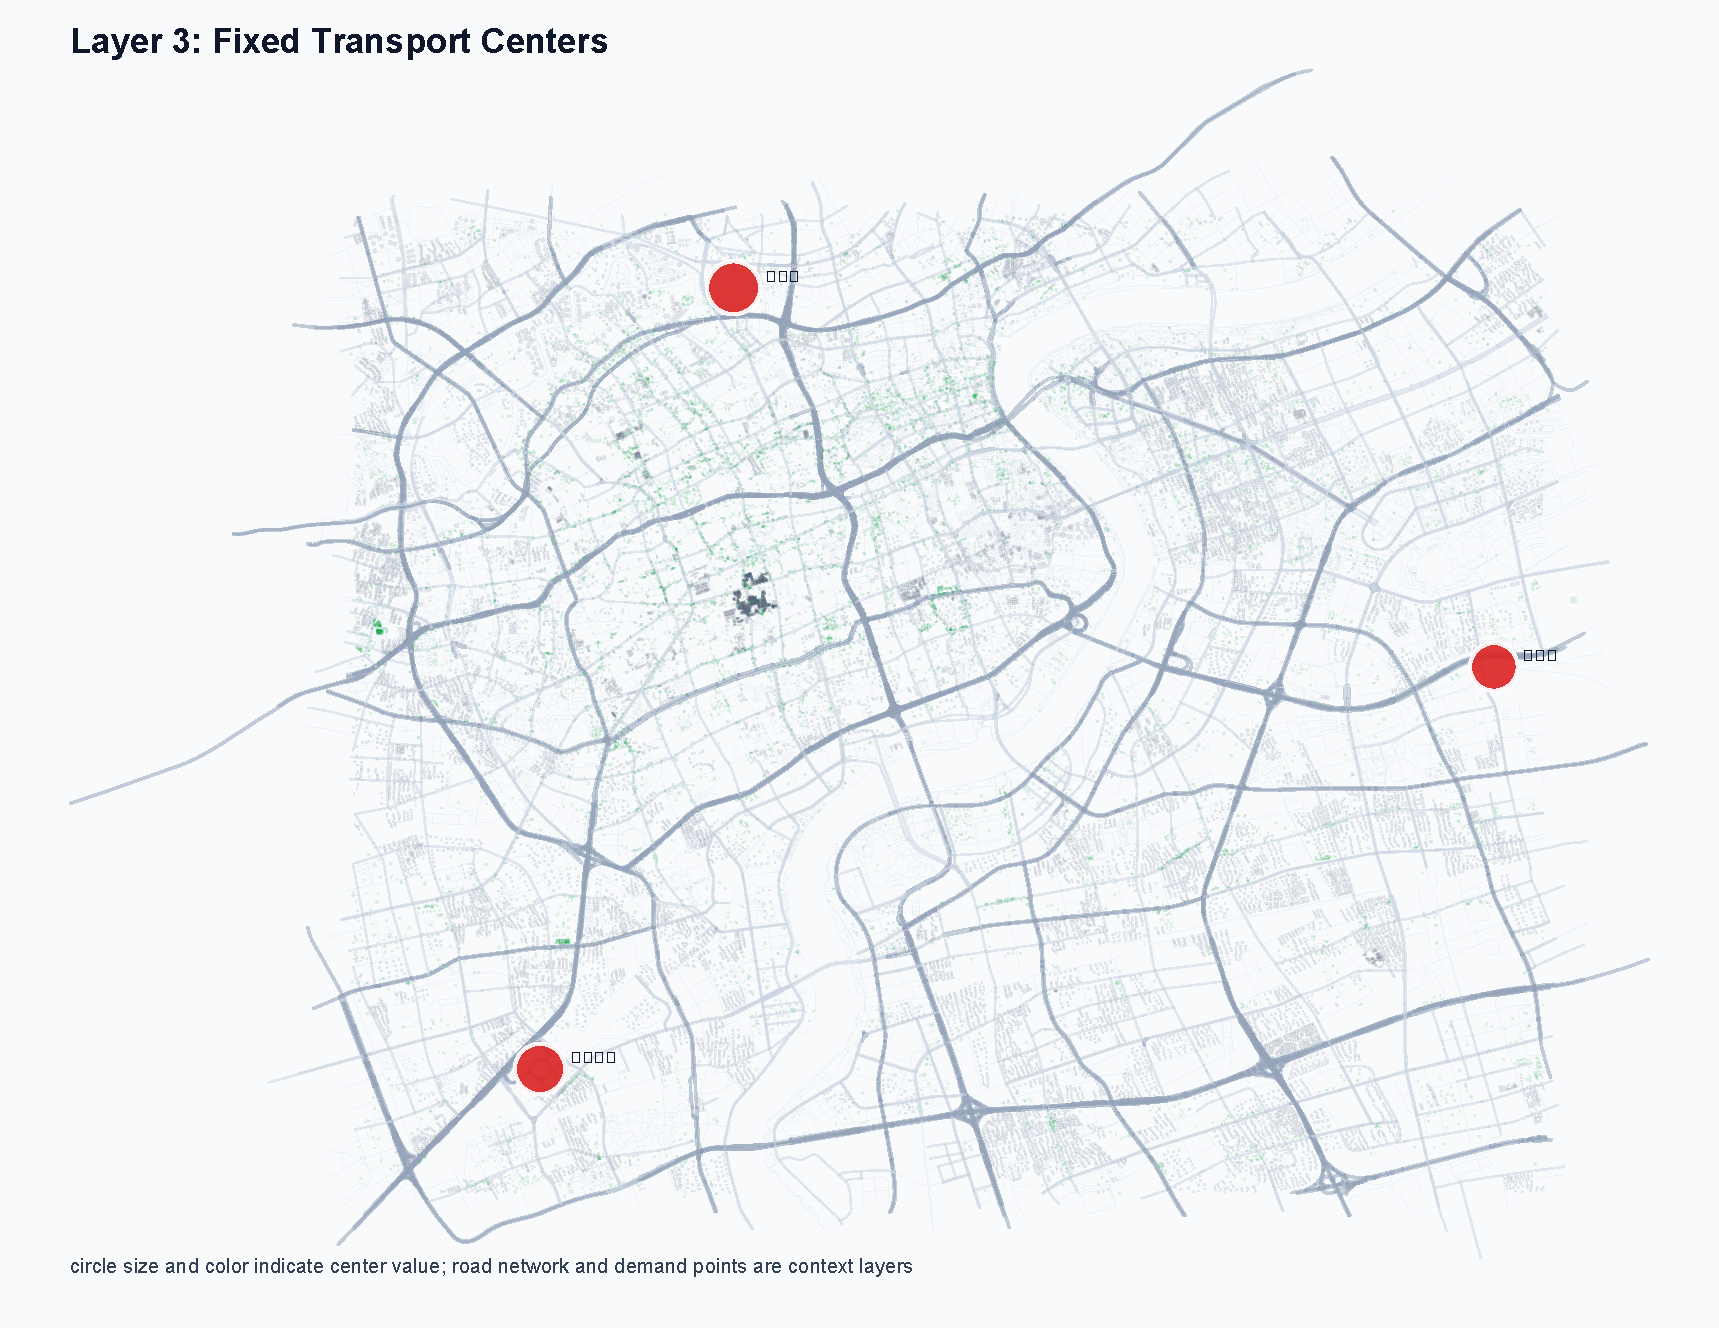
\includegraphics[width=\linewidth]{figures/01c_transport_centers.pdf}
            \caption*{(c) Transport centers}
        \end{minipage}
        \hfill
        \begin{minipage}{0.49\textwidth}
            \centering
            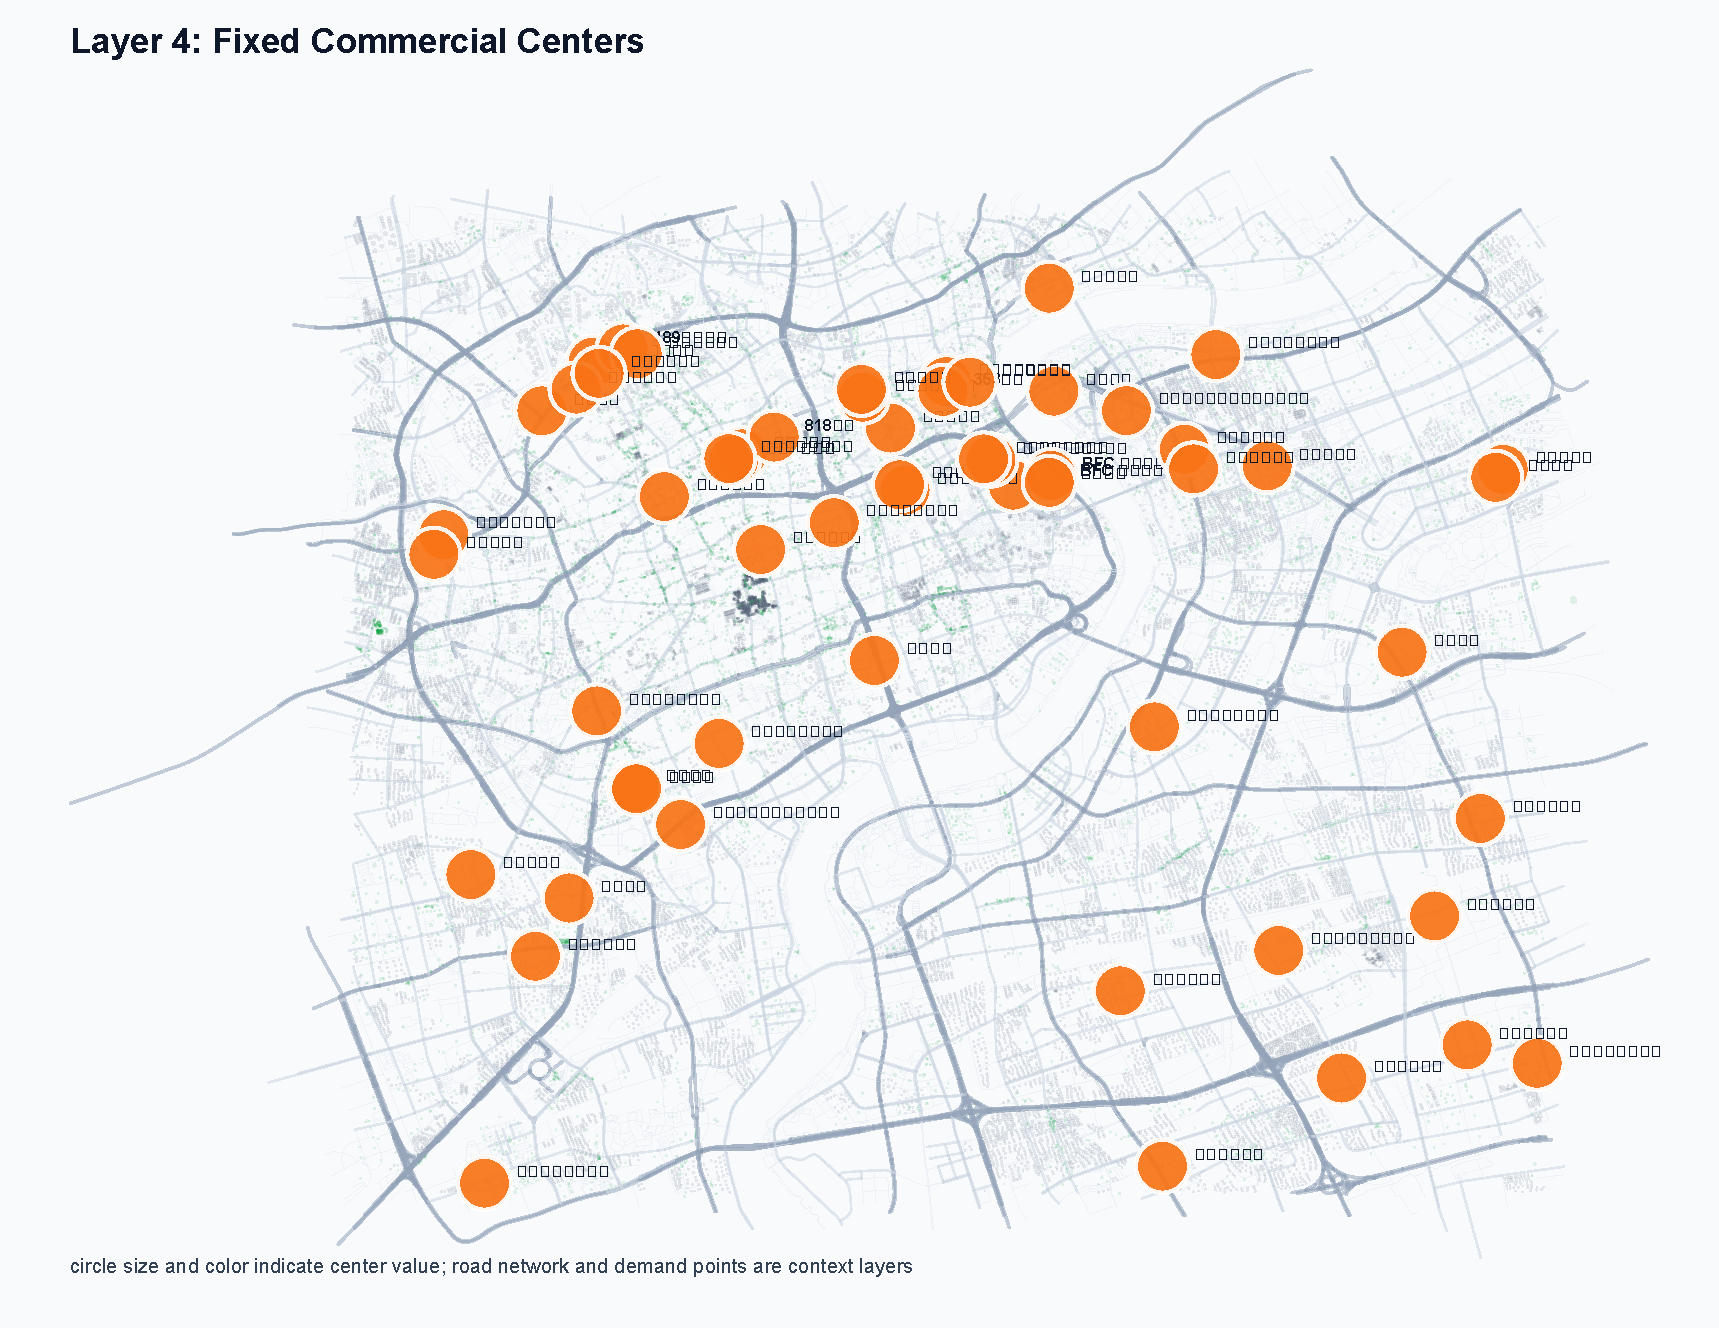
\includegraphics[width=\linewidth]{figures/01d_commercial_centers.pdf}
            \caption*{(d) Large commercial centers}
        \end{minipage}
        \caption{Four center layers used to construct candidate stations.}
        \label{fig:center-layers}
    \end{figure*}

    After the four center layers are generated, nearby centers are merged to avoid creating several candidate stations for the same urban cluster. Centers within 1,000 meters are combined into one candidate station, whose location is the value-weighted centroid of its components. The station value is additive:
    \[
        v_i =
        v_i^{\mathrm{pop}} +
        v_i^{\mathrm{job}} +
        v_i^{\mathrm{trans}} +
        v_i^{\mathrm{comm}}.
    \]
    The merge radius also acts as a minimum spacing rule. In the current study area, the preprocessing stage merges the four layers into 54 candidate stations. These candidate stations become the input vertices for the route-design algorithms.

    \begin{figure*}[t]
        \centering
        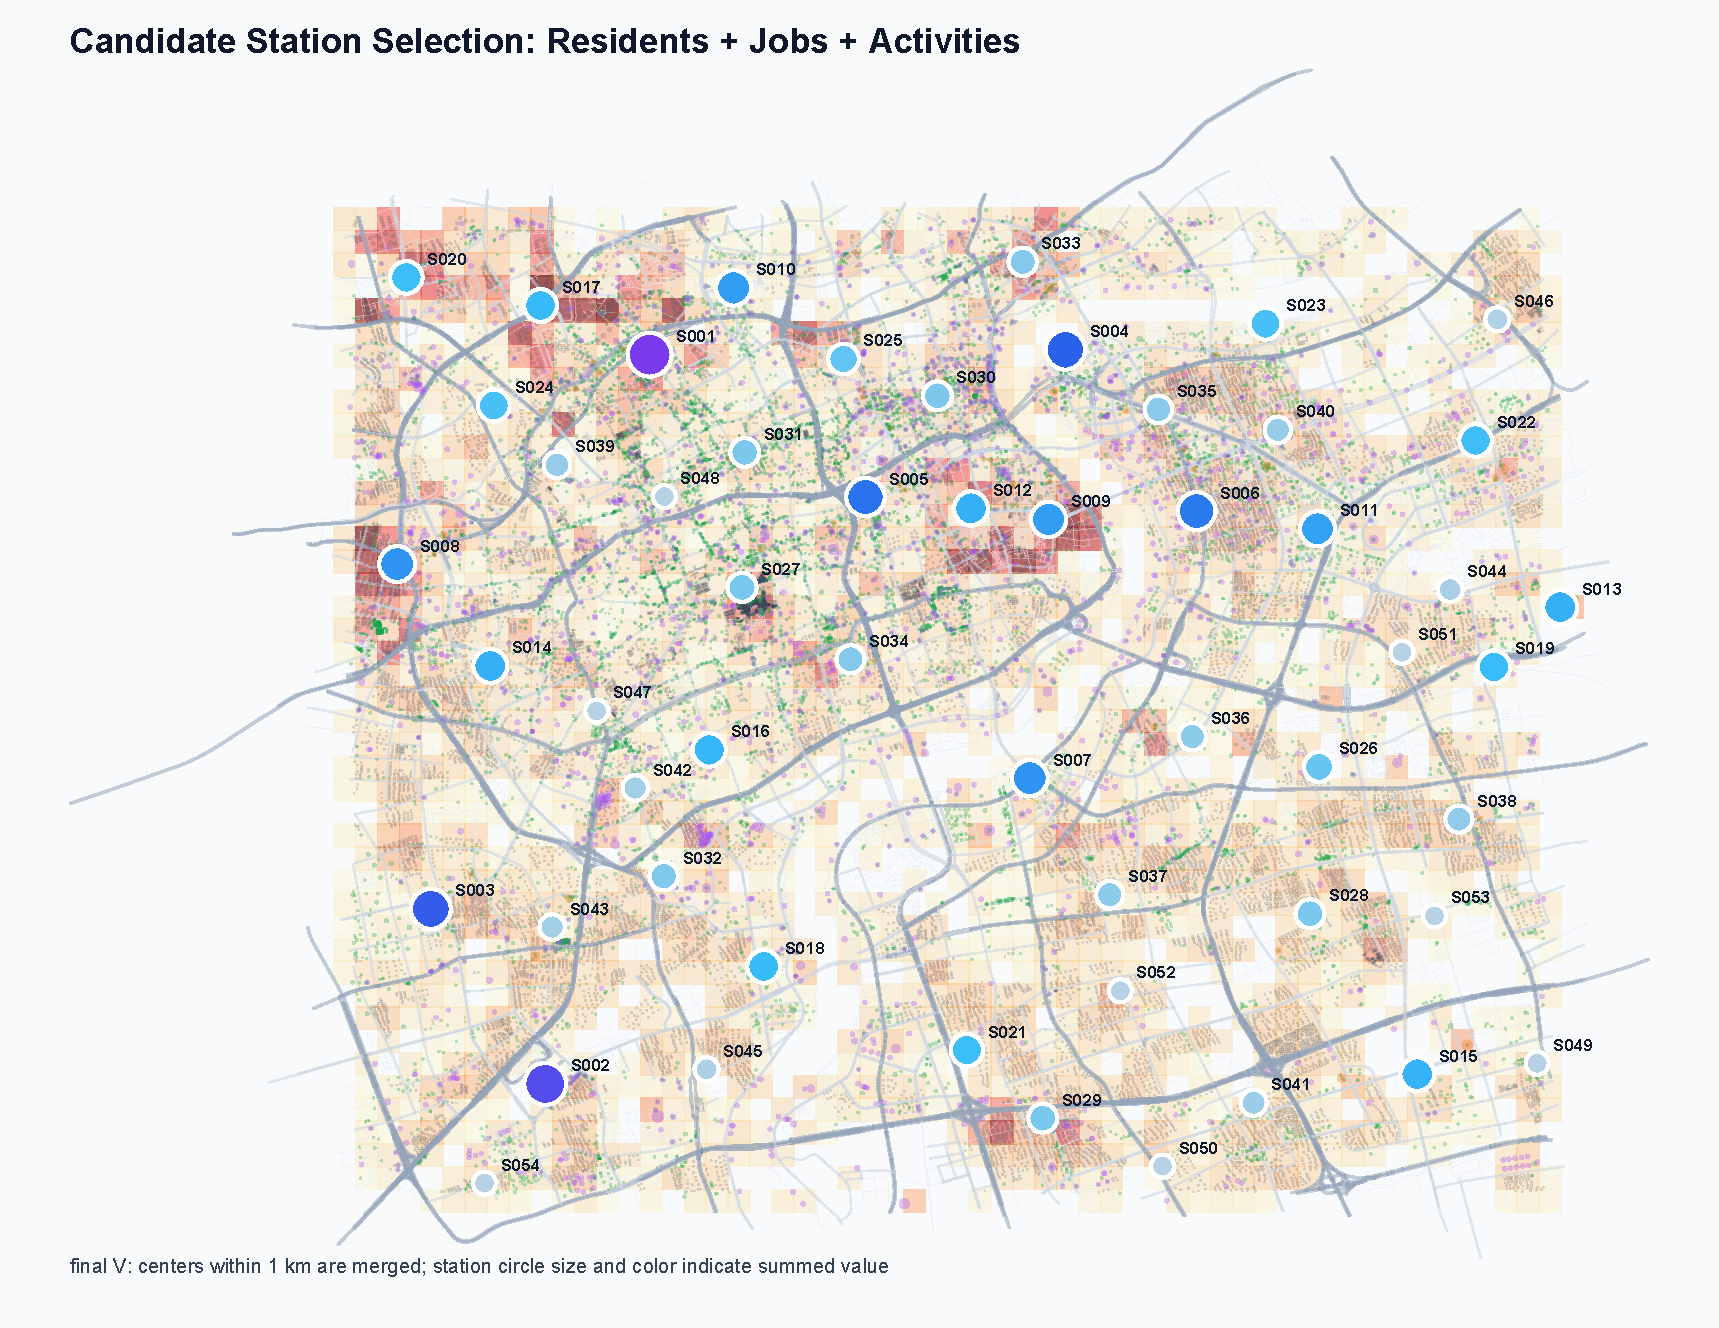
\includegraphics[width=0.94\textwidth]{figures/01_station_selection.pdf}
        \caption{Final candidate-station set after merging nearby centers from the four data layers.}
        \label{fig:station-selection}
    \end{figure*}

    Existing Shanghai metro lines are used only as a visual reference for plausibility checks. They are not mandatory stops or fixed edges in the optimization model.

\section{Algorithm and Technical Plan}

    We plan to study three algorithmic approaches. They share the same candidate stations, station values, edge lengths, pairwise connection reward, construction-cost penalty, turn-angle penalty, and endpoint penalty. The methods differ mainly in how explicitly they model metro lines.

    The first method is a greedy prize-collecting network heuristic with leaf pruning. It starts from a high-scoring station pair, repeatedly adds the station-edge connection with the best marginal gain, and then removes low-benefit terminal leaves if doing so improves the full penalized objective. This gives a simple classical baseline that is easy to inspect and tune.

    The second method searches directly over a small number of metro paths. It first generates promising smooth paths between high-value terminal pairs using a bounded shortest-path or beam-search procedure, then selects a set of paths whose union maximizes the objective. This approach is less exact than mathematical programming, but its outputs are naturally interpretable as metro lines.

    The third method is a small-instance integer or mixed-integer programming benchmark. Binary variables represent selected stations, selected edges, pair connections, and line membership, with additional constraints for connectivity, endpoints, and turn transitions. Because the full problem is NP-hard and the shortest-path reward depends on the selected network, this model is intended mainly for validating heuristic results on smaller candidate sets.

\section{Project Scope and Expected Goals}

    The core scope of this project is to build and evaluate an algorithmic pipeline for generating candidate Shanghai metro corridors from public spatial data. The main optimization goal is to maximize the penalized value-connection objective defined above. In other words, the primary output should be a selected set of stations and edges, or a small set of line paths, that connects high-value urban centers while controlling construction length, sharp turns, and excessive terminal endpoints. The project therefore emphasizes explainable network-design algorithms rather than a complete professional ridership forecasting system.

    Within this scope, our expected goals are threefold. First, we will construct a reproducible data pipeline that converts population, employment, transport-center, and commercial-center information into a discrete candidate-station set. Second, we will compare several optimization methods, including the greedy PCST-style baseline, multi-path search, and a small-scale integer-programming benchmark. Third, we will evaluate the resulting networks with interpretable metrics such as selected station count, total construction length, pairwise connection reward, turn penalty, endpoint penalty, and visual plausibility relative to existing Shanghai metro corridors.

    Beyond maximizing the objective value itself, we may further analyze passenger-flow intensity if suitable data or a reasonable proxy becomes available. In a more detailed evaluation stage, the selected network can be combined with a synthetic travel-demand estimate derived from population, employment, land use, and travel-time impedance. Passenger demand can then be assigned to the generated metro network using shortest-path or flow-assignment rules. This would allow us to estimate section-level passenger volumes rather than only station-level value scores.

    A particularly useful downstream metric is the maximum section passenger flow, which is the largest passenger volume carried by any edge or line segment in the planned network. This metric is widely used in transit planning because it reflects the most heavily loaded part of a line and is closely related to capacity planning, train frequency, and bottleneck detection. If observed passenger-flow or maximum-section-flow data for Shanghai metro lines can be obtained, we can use it to compare the generated corridors with real operating patterns. If such data is unavailable, we can still compute synthetic section loads from the estimated demand and use them as a relative evaluation measure.

    Therefore, the minimum expected outcome is an optimized and interpretable candidate-line network under the proposed objective. A stronger outcome would add passenger-flow analysis on top of the selected network: estimating synthetic travel demand, assigning it to paths, reporting section passenger intensity, and identifying the maximum-load segment. This extension would not replace the graph-optimization objective, but would help test whether the mathematically high-scoring network also makes sense from an operational passenger-demand perspective.
    
\section{Team Information}

    The project team consists of three members. We expect the work to be divided by pipeline stage and technical responsibility, while keeping the final formulation, experiments, and writing jointly reviewed by all members.

    \begin{itemize}
        \item \textbf{Yuzhou Lu}: Responsible for literature review, problem framing, and formulation refinement. Expected contributions include connecting the project to TNDP and prize-collecting network design literature, clarifying modeling assumptions, and helping write the proposal and final report.
        \item \textbf{Zaizhou Yang}: Responsible for data pipeline construction and algorithm implementation. Expected contributions include preparing OSM-based population, employment, transport-center, and commercial-center inputs; implementing the greedy baseline and later optimization methods; and generating maps and quantitative outputs.
        \item \textbf{Jingrong Guan}: Responsible for evaluation design, passenger-flow analysis, and experimental comparison. Expected contributions include defining evaluation metrics, analyzing objective values and line-network geometry, exploring synthetic demand assignment, and comparing section passenger intensity or maximum-section-flow indicators when data is available.
    \end{itemize}

    In addition to these primary roles, all team members will participate in debugging, result interpretation, presentation preparation, and final editing. This division is intended to make each component accountable while preserving enough overlap for cross-checking the model and experiments.

%----------------------------------------------------------

\printbibliography

%----------------------------------------------------------

\end{document}
